%%%%%%%%%%%%%%%%%%%%%%%%%%%%%%%%%%%%%%%%%%%%%%%%%%%%%%%%%%%%%%%%%%%%%%%%%%%%%%%%
% TUM-Vorlage: Wissenschaftliche Arbeit
%%%%%%%%%%%%%%%%%%%%%%%%%%%%%%%%%%%%%%%%%%%%%%%%%%%%%%%%%%%%%%%%%%%%%%%%%%%%%%%%
%
% Rechteinhaber:
%     Technische Universität München
%     https://www.tum.de
% 
% Gestaltung:
%     ediundsepp Gestaltungsgesellschaft, München
%     http://www.ediundsepp.de
% 
% Technische Umsetzung:
%     eWorks GmbH, Frankfurt am Main
%     http://www.eworks.de
%
%%%%%%%%%%%%%%%%%%%%%%%%%%%%%%%%%%%%%%%%%%%%%%%%%%%%%%%%%%%%%%%%%%%%%%%%%%%%%%%%

%%%%%%%%%%%%%%%%%%%%%%%%%%%%%%%%%%%%%%%%%%%%%%%%%%%%%%%%%%%%%%%%%%%%%%%%%%%%%%%%
\documentclass[10pt]{scrlttr2} % Dokumentenklasse: KOMA-Skript Letter

% Anpassbare Kopf- und Fußzeilen für KOMA-Skript:
%\usepackage{scrlayer-scrpage}

\usepackage[utf8]{inputenc} % Textkodierung: UTF-8
\usepackage[T1]{fontenc} % Zeichensatzkodierung

\usepackage{calc} % Berechnungen

\usepackage[ngerman]{babel} % Deutsche Lokalisierung
\usepackage{graphicx} % Grafiken
\usepackage[absolute]{textpos} % Positionierung

% Silbentrennung:
\usepackage{hyphenat}
%\tolerance 2414
%\hbadness 2414
%\emergencystretch 1.5em
%\hfuzz 0.3pt
%\widowpenalty=10000     % Hurenkinder
%\clubpenalty=10000      % Schusterjungen
%\vfuzz \hfuzz

% Euro-Symbol:
\usepackage[gen]{eurosym}
\DeclareUnicodeCharacter{20AC}{\euro{}}

% Schriftart Helvetica:
\usepackage[scaled]{helvet}
\renewcommand{\familydefault}{\sfdefault}

\usepackage{mathptmx} % skalierbare Formelschriften
\usepackage{xstring} % Textmanipulation
\usepackage{xcolor} % Farbdefinitionen

\usepackage{etoolbox} % Toggle-Definitionen
\newtoggle{StellenausschreibungGrafikOpportunities}
\togglefalse{StellenausschreibungGrafikOpportunities}

% Debugging:
%\usepackage{layout} % Layout-Informationen
%\usepackage{printlen} % Längenwerte ausgeben
 % !!! NICHT ENTFERNEN !!!
%%%%%%%%%%%%%%%%%%%%%%%%%%%%%%%%%%%%%%%%%%%%%%%%%%%%%%%%%%%%%%%%%%%%%%%%%%%%%%%%

\renewcommand{\Thema}{%
    Thema der Arbeit (optional)}

%%%%%%%%%%%%%%%%%%%%%%%%%%%%%%%%%%%%%%%%%%%%%%%%%%%%%%%%%%%%%%%%%%%%%%%%%%%%%%%%
%%%%%%%%%%%%%%%%%%%%%%%%%%%%%%%%%%%%%%%%%%%%%%%%%%%%%%%%%%%%%%%%%%%%%%%%%%%%%%%%
% EINSTELLUNGEN
%%%%%%%%%%%%%%%%%%%%%%%%%%%%%%%%%%%%%%%%%%%%%%%%%%%%%%%%%%%%%%%%%%%%%%%%%%%%%%%%

% Allgemein:
\newcommand{\AllgemeinGestalter}{ediundsepp Gestaltungsgesellschaft}
\newcommand{\AllgemeinErsteller}{eWorks GmbH}

% Universität:
\newcommand{\UniversitaetName}{Technische Universität München}
\newcommand{\UniversitaetAbkuerzung}{TUM}
\newcommand{\UniversitaetWebseite}{www.tum.de}
\newcommand{\UniversitaetLogoBreite}{19mm}
\newcommand{\UniversitaetLogoHoehe}{1cm}

\newcommand{\UniversitaetAdresse}{%
    Arcisstraße~21\\%
    80333~München%
}


% Seitenränder:
\newcommand{\SeitenrandOben}{20mm}
\newcommand{\SeitenrandRechts}{20mm}
\newcommand{\SeitenrandLinks}{25mm}
\newcommand{\SeitenrandUnten}{10mm}

% Falzmarken:
\newcommand{\FalzmarkeOben}{87mm}
\newcommand{\FalzmarkeMitte}{148.5mm}
\newcommand{\FalzmarkeUnten}{192mm}
\newcommand{\FalzmarkeBreite}{2mm}
\newcommand{\FalzmarkeDicke}{0.3pt}
\newcommand{\FalzmarkePositionLinks}{7mm}


% Adressfeld:
\newcommand{\AdressfeldHoehe}{45mm}
\newcommand{\AdressfeldBreite}{85mm}
\newcommand{\AdressfeldAbsenderSchriftgroesse}{7.5pt}
\newcommand{\AdressfeldEmpfaengerSchriftgroesse}{11pt}
\newcommand{\AdressfeldEmpfaengerZeilenabstand}{15pt}

% Text:
\newcommand{\TextOben}{77.5mm}
\newcommand{\TextSchriftgroesse}{11pt}
\newcommand{\TextZeilenabstand}{15pt}

% Fusszeile:
\newcommand{\FusszeilePositionOben}{271mm}
\newcommand{\FusszeileBreite}{165mm}
\newcommand{\FusszeileHoehe}{16.5mm}
\newcommand{\FusszeileZwischenabstand}{2mm}
\newcommand{\FusszeileBreiteGross}{44mm}
\newcommand{\FusszeileBreiteKlein}{35.5mm}
\newcommand{\FusszeileSeitennummerAbstand}{7.7mm}
\newcommand{\FusszeileSchriftgroesse}{7.5pt}
\newcommand{\FusszeileZeilenabstand}{8pt}


%%%%%%%%%%%%%%%%%%%%%%%%%%%%%%%%%%%%%%%%%%%%%%%%%%%%%%%%%%%%%%%%%%%%%%%%%%%%%%%%
% DOKUMENT
%%%%%%%%%%%%%%%%%%%%%%%%%%%%%%%%%%%%%%%%%%%%%%%%%%%%%%%%%%%%%%%%%%%%%%%%%%%%%%%%

\usepackage[a4paper,
    top=\SeitenrandOben,
    bottom=\SeitenrandUnten,
    inner=\SeitenrandLinks,
    outer=\SeitenrandRechts,
    foot=\FusszeileHoehe - 1mm,
    head=0cm,
    includefoot
]{geometry}

\textblockorigin{\SeitenrandLinks}{\SeitenrandOben} % Ursprung für Positionierung

% PDF-Einstellungen:
\usepackage[pdftex]{hyperref}
\hypersetup{
    hidelinks,
    pdfauthor={\PersonVorname{} \PersonNachname},
    pdftitle={\Betreff},
    pdfproducer={\AllgemeinErsteller},
    pdfcreator={\AllgemeinGestalter}
}

\renewcommand*{\raggedsignature}{\raggedright}

\makeatletter
    \@setplength{bfoldmarklength}{\FalzmarkeBreite}
    \@setplength{bfoldmarkvpos}{\FalzmarkeUnten}
    \@setplength{firstfoothpos}{\SeitenrandLinks - 2pt}
    \@setplength{firstfootvpos}{\FusszeilePositionOben}
    \@setplength{firstfootwidth}{\FusszeileBreite}
    \@setplength{foldmarkhpos}{\FalzmarkePositionLinks}
    \@setplength{foldmarkthickness}{\FalzmarkeDicke}
    \@setplength{mfoldmarklength}{\FalzmarkeBreite}
    \@setplength{mfoldmarkvpos}{\FalzmarkeMitte}

    \@setplength{refaftervskip}{\TextZeilenabstand}
    \@setplength{refvpos}{\TextOben}
    \@setplength{sigbeforevskip}{\baselineskip}
    \@setplength{sigindent}{0mm}
    \@setplength{subjectaftervskip}{\baselineskip + \baselineskip + 1pt}

    \@setplength{tfoldmarklength}{\FalzmarkeBreite}
    \@setplength{tfoldmarkvpos}{\FalzmarkeOben}
\makeatother

\KOMAoptions{
    fontsize=\TextSchriftgroesse,
    foldmarks=BMpTv,
    firsthead=false,
    backaddress=no,
    addrfield=no,
    fromalign=false
}

\setkomavar{fromname}{\UniversitaetName}
\setkomavar{fromaddress}{\PersonAdresse}
\addtokomafont{backaddress}{\fontsize{\AdressfeldAbsenderSchriftgroesse}{\AdressfeldAbsenderSchriftgroesse}\selectfont}
\addtokomafont{toaddress}{\fontsize{\AdressfeldEmpfaengerSchriftgroesse}{\AdressfeldEmpfaengerZeilenabstand}\selectfont}

\newcommand{\RuecksendeadresseTrenner}{~| \ignorespaces}

\AtBeginLetter{%
    % Logo:
    \begin{textblock*}{\UniversitaetLogoBreite}[1,0](\textwidth, 0cm)%
        \raggedleft%
        
\includegraphics{./Ressourcen/_Bilder/Universitaet_Logo_RGB.pdf}%
    \end{textblock*}%
    \setlength{\baselineskip}{\TextZeilenabstand}%
    \setlength{\parindent}{0mm} % keine Einrückung am Absatzanfang
    \setlength{\parskip}{\baselineskip} % einzeiliger Abstand nach Absätzen
    % Empfängerfenster:
    \begin{textblock*}{\AdressfeldBreite}[0,0](0cm, 15mm)%
        \raggedbottom\raggedright
        \begin{spacing}{.85}%
        {
            \usekomafont{backaddress}%
            \let\\\RuecksendeadresseTrenner% Umdefinieren von "\\" zu "~| "
            \Absender%
        } \\
        \end{spacing}
        \vspace*{5.5pt}
        \usekomafont{toaddress}%
        \EmpfaengerAdresse
    \end{textblock*}
}

\KOMAoptions{refline=dateleft}
\setkomavar{date}{\Datum}
\setkomavar{place}{\PersonStadt}
\setkomafont{subject}{\bfseries}
\setkomavar{subject}{\Betreff}
\setkomavar{signature}{\PersonVorname~\PersonNachname}

%\setkomavar*{enclseparator}{Anlage\vspace{-3em}}

\renewcommand*{\closing}[1]{#1\vspace*{3\baselineskip}\newline\usekomavar{signature}\newline}
\setkomavar{enclseparator}[Anlage]{~}
\renewcommand{\encl}[1]{\newline{}Anlage~#1}

\KOMAoptions{firstfoot=true}
\setkomafont{pagefoot}{\sffamily\fontsize{7.5pt}{8pt}\selectfont}
\renewcommand{\pagemark}{%
\begin{textblock*}{3em}[1,1](\paperwidth - \SeitenrandLinks - \SeitenrandRechts + \FusszeileSeitennummerAbstand + 3mm, \paperheight - \SeitenrandOben - \SeitenrandUnten)%
    \raggedleft\hfill\usekomafont{pagefoot}\thepage\,/\,\pageref*{LastPage}%
\end{textblock*}%
}

\setkomavar{firstfoot}{
    \TabPositions{2em}%
    \begin{minipage}[t][\FusszeileHoehe][t]{\FusszeileBreiteGross}%
        \usekomafont{pagefoot}%
        \textbf{\UniversitaetName}%
        \newline%
        \FakultaetName%
        \newline%
        \LehrstuhlName%
    \end{minipage}%
    \hspace*{\FusszeileZwischenabstand}%
    \begin{minipage}[t][\FusszeileHoehe][t]{\FusszeileBreiteGross}%
        \raggedright\usekomafont{pagefoot}%
        \textbf{\FakultaetAnsprechpartner}\newline%
        \PersonAdresse%
    \end{minipage}%
    \hspace*{\FusszeileZwischenabstand}%
    \begin{minipage}[t][\FusszeileHoehe][t]{\FusszeileBreiteKlein}%
        \raggedright\usekomafont{pagefoot}%
        Tel.\tab{\PersonTelefon}%
        \def\temp{\PersonFax}\ifx\temp\empty%
        \else%
          \newline Fax\tab{\PersonFax}%
        \fi%
        \newline\newline%
        \PersonEmail\newline%
        \href{http://\PersonWebseite}{\PersonWebseite}\newline%
        \href{http://\UniversitaetWebseite}{\UniversitaetWebseite}%
    \end{minipage}%
    \hspace*{\FusszeileZwischenabstand}%
    \begin{minipage}[t][\FusszeileHoehe][t]{\FusszeileBreiteKlein}%
        \raggedright\usekomafont{pagefoot}%
        \EinstellungBankName\newline%
        IBAN-Nr.: \EinstellungBankIBAN\newline%
        BIC: \EinstellungBankBIC\newline%
        Steuer-Nr.: \EinstellungSteuernummer\newline%
        USt-IdNr.: \EinstellungUmsatzsteuerIdentifikationsnummer\newline%
    \end{minipage}%
    \pagemark%
}

\begin{document}
\raggedright
\begin{letter}{\EmpfaengerAdresse{}}
\opening{\Gruss}

 % !!! NICHT ENTFERNEN !!!
%%%%%%%%%%%%%%%%%%%%%%%%%%%%%%%%%%%%%%%%%%%%%%%%%%%%%%%%%%%%%%%%%%%%%%%%%%%%%%%%

\begin{document}

\title{Thema der Arbeit}
\author{Martin Mustermann}
\date{Datum}


\tableofcontents % Inhaltsverzeichnis

\chapter{Kapitelüberschrift}

\section{Unterkapitelüberschrift}

\subsection[]{Absatzüberschrift}

Dies ist die Vorlage für eine wissenschaftliche Arbeit nach dem Corporate
Design der Technischen Universität München (TUM). Die Vorlage ist für "`TeX
Live 2015"' kompatibel.

Bitte geben Sie Ihren individuellen Text an den vorgesehenen Stellen ein und
beachten Sie die Formatvorgaben des jeweiligen Lehrstuhls oder der Prüfenden
zum inhaltlichen und formalen Aufbau der wissenschaftlichen Arbeit. Achten Sie
grundsätzlich auf ein angenehmes Erscheinungsbild für den Leser und dass ein
1,5-facher Zeilenabstand und am Rand genügend Platz für Korrekturen
eingehalten wird\footnote{Bitte beachten Sie die Zitationsvorgaben Ihres
Prüfers.}.

Grundsätzlich sind die Schriftarten Arial und Times New Roman, sowie die Neue
Helvetica zulässig. Der Text ist links ausgerichtet und in Blocksatz gesetzt.
Auszeichnungen der Schrift können durch Fettung, Schrägstellung und
Unterstreichung erfolgen. Farbige Schrift sollte nur in Ausnahmefällen oder
Grafiken zum Einsatz kommen.

\begin{figure}[!ht]
\noindent\hspace{0.5mm}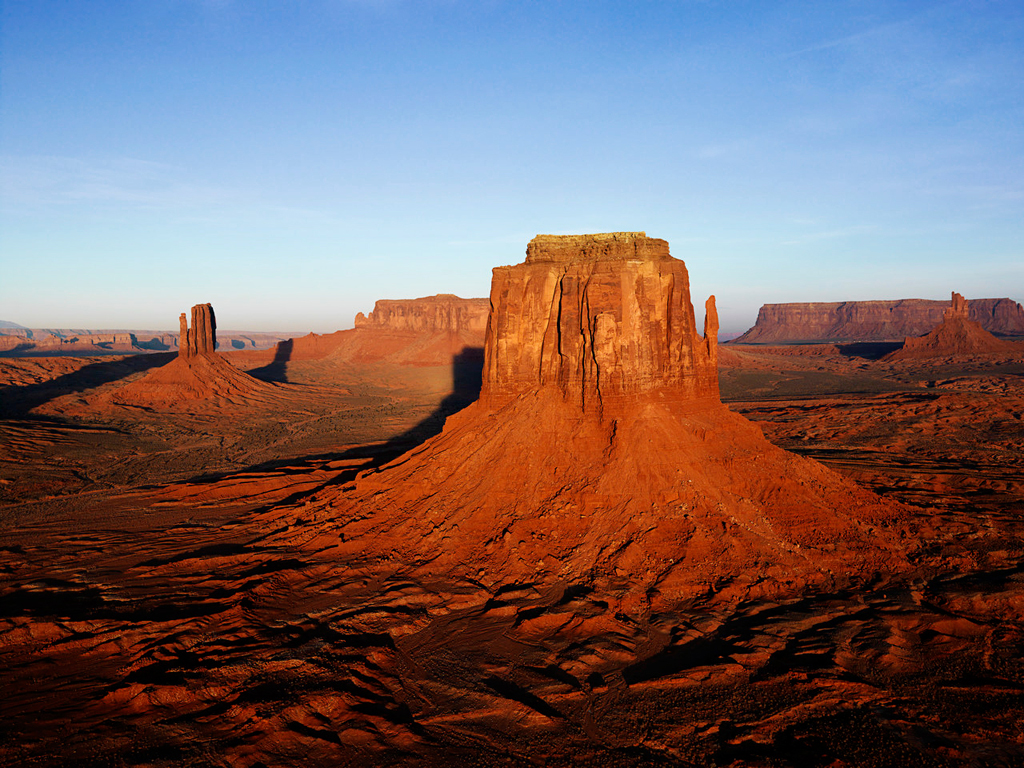
\includegraphics[width=12cm]{./Ressourcen/Desert.jpg}
\caption{Titel, Autor}
\end{figure}

\clearpage

Passen Sie gegebenenfalls die Ränder an die Vorgaben Ihres Prüfers an und
beachten Sie dabei, dass das Logo der TUM sich oben rechts innerhalb der
Ränder, auf der Titelseite befindet. Für die Titelseiten stehen separate
Vorlagen zur Verfügung.

Zur Definition von \gls{abk} erstellen Sie für die gewünschte Abkürzung einen
Eintrag in der Datei \texttt{Abkuerzungen.tex} und referenzieren sie ihn
mittels \texttt{\textbackslash{}gls}; diese tauchen nach einem Lauf mit
\texttt{latexmk} im Abkürzungsverzeichnis auf. Beispiel:

\vspace{-\baselineskip}
\begin{description}[leftmargin=1em+5mm, labelindent=5mm]
\item[Definition in \texttt{Abkuerzungen.tex}:] \texttt{\textbackslash{}newacronym\{abk\}\{Abk.\}\{Abkürzungen\}\}}
\item[Referenzierung:] \texttt{\textbackslash{}gls\{abk\}}
\end{description}

Für weitere Informationen zu Glossaren und Abkürzungen siehe die Dokumentation
des Pakets \texttt{glossaries} und die entsprechenden Abschnitte in den
Vorlagendateien.


\subsection[]{Aufzählungen}

\begin{itemize}
\item Dies ist die Standardaufzählung
    \begin{itemize}
    \item Dies ist die nächste Ebene der Aufzählung
    \end{itemize}
\end{itemize}


\subsection[]{Nummerierungen}

\begin{enumerate}
\item Erster Punkt der Nummerierungen
    \begin{enumerate}
    \item Unterpunkt der Nummerierungen
    \end{enumerate}
\end{enumerate}
\clearpage

\listoffigures % Abbildungsverzeichnis

\printacronyms[title={Abkürzungsverzeichnis}] % Abkürzungsverzeichnis

\listoftables % Tabellenverzeichnis

\onehalfspacing

\addchap{Tabellenvarianten}

\vspace{22mm}
\section*{Überschrift Tabelle 1}

\begin{table}[!h]
\begin{tabularx}{\textwidth + 5pt}{@{\hspace{3pt}} M | @{\hspace{3pt}} M}
\multicolumn{2}{@{}X}{%
    \begin{tabularx}{\textwidth}{@{\hspace{3pt}} M @{\hspace{14.5pt}} M}
    \textbf{Spalte 1} & \textbf{Spalte 2}
    \end{tabularx}%
} \\
\hline
Nummer 1 & Nummer 2 \\
\hline
Nummer 1 & Nummer 2 \\
\hline
Nummer 1 & Nummer 2 \\
\hline
\end{tabularx}

\caption{Beschreibung}
\end{table}


\vspace{\parskip}
\section*{Überschrift Tabelle 2}

\begin{table}[!h]
\hspace{-5pt}
\begin{tabularx}{\textwidth + 5pt}{| @{\hspace{3pt}} M | @{\hspace{3pt}} M |}
\hline
\textbf{Spalte 1} & \textbf{Spalte 2} \\
\hline
Nummer 1 & Nummer 2 \\
\hline
Nummer 1 & Nummer 2 \\
\hline
Nummer 1 & Nummer 2 \\
\hline
\end{tabularx}
\caption{}
\end{table}


\vspace{\parskip}
\section*{Überschrift Tabelle 3}

\begin{table}[!h]
\begin{tabularx}{\textwidth}{@{} M M}
\textbf{Spalte 1} & \textbf{Spalte 2} \\
Nummer 1 & Nummer 2 \\
Nummer 1 & Nummer 2 \\
Nummer 1 & Nummer 2 \\
\end{tabularx}
\caption{}
\end{table}

\clearpage

\addchap{Tabellenvarianten 2}

\vspace{22mm}
\section*{Überschrift Tabelle 1}

\begin{table}[!h]
\fontsize{9pt}{13pt}\selectfont
%\renewcommand{\arraystretch}{1.8}
\hspace{-5pt}
\begin{tabularx}{\textwidth + 5pt}{@{\hspace{3pt}} M | @{\hspace{3pt}} M}
\multicolumn{2}{@{}X}{%
    \begin{tabularx}{\textwidth}{@{\hspace{3pt}} M @{\hspace{14.5pt}} M}
    \textbf{Spalte 1} & \textbf{Spalte 2}
    \end{tabularx}%
} \\
\hline
Nummer 1,\newline\,mehrzeilig in Schriftgröße 9 pt & Nummer 2 \\
\hline
Nummer 1 & Nummer 2 \\
\hline
Nummer 1 & Nummer 2 \\
\hline
\end{tabularx}

\caption{}
\end{table}


\vspace{\parskip}
\section*{Überschrift Tabelle 2}

\begin{table}[!h]
\fontsize{9pt}{13pt}\selectfont
\hspace{-5pt}
%\renewcommand{\arraystretch}{1.8}
\begin{tabularx}{\textwidth + 5pt}{| @{\hspace{3pt}} M | @{\hspace{3pt}} M |}
\hline
\textbf{Spalte 1} & \textbf{Spalte 2} \\
\hline
Nummer 1 & Nummer 2 \\
\hline
Nummer 1 & Nummer 2 \\
\hline
Nummer 1 & Nummer 2 \\
\hline
\end{tabularx}
\caption{}
\end{table}


\vspace{\parskip}
\section*{Überschrift Tabelle 3}

\begin{table}[!h]
\fontsize{9pt}{13pt}\selectfont
%\renewcommand{\arraystretch}{1.8}
\begin{tabularx}{\textwidth}{@{} M M}
\textbf{Spalte 1} & \textbf{Spalte 2} \\
Nummer 1 & Nummer 2 \\
Nummer 1 & Nummer 2 \\
Nummer 1 & Nummer 2 \\
\end{tabularx}
\caption{}
\end{table}

\end{document}